\documentclass[12pt,letterpaper]{article}
\usepackage{graphicx,textcomp}
\usepackage{natbib}
\usepackage{setspace}
\usepackage{fullpage}
\usepackage{color}
\usepackage[reqno]{amsmath}
\usepackage{amsthm}
\usepackage{fancyvrb}
\usepackage{amssymb,enumerate}
\usepackage[all]{xy}
\usepackage{endnotes}
\usepackage{lscape}
\newtheorem{com}{Comment}
\usepackage{float}
\usepackage{hyperref}
\newtheorem{lem} {Lemma}
\newtheorem{prop}{Proposition}
\newtheorem{thm}{Theorem}
\newtheorem{defn}{Definition}
\newtheorem{cor}{Corollary}
\newtheorem{obs}{Observation}
\usepackage[compact]{titlesec}
\usepackage{dcolumn}
\usepackage{tikz}
\usetikzlibrary{arrows}
\usepackage{multirow}
\usepackage{xcolor}
\newcolumntype{.}{D{.}{.}{-1}}
\newcolumntype{d}[1]{D{.}{.}{#1}}
\definecolor{light-gray}{gray}{0.65}
\usepackage{url}
\usepackage{listings}
\usepackage{color}

\definecolor{codegreen}{rgb}{0,0.6,0}
\definecolor{codegray}{rgb}{0.5,0.5,0.5}
\definecolor{codepurple}{rgb}{0.58,0,0.82}
\definecolor{backcolour}{rgb}{0.95,0.95,0.92}

\lstdefinestyle{mystyle}{
	backgroundcolor=\color{backcolour},   
	commentstyle=\color{codegreen},
	keywordstyle=\color{magenta},
	numberstyle=\tiny\color{codegray},
	stringstyle=\color{codepurple},
	basicstyle=\footnotesize,
	breakatwhitespace=false,         
	breaklines=true,                 
	captionpos=b,                    
	keepspaces=true,                 
	numbers=left,                    
	numbersep=5pt,                  
	showspaces=false,                
	showstringspaces=false,
	showtabs=false,                  
	tabsize=2
}
\lstset{style=mystyle}
\newcommand{\Sref}[1]{Section~\ref{#1}}
\newtheorem{hyp}{Hypothesis}

\title{Problem Set 2}
\date{Due: October 16, 2022}
\author{Applied Stats/Quant Methods 1}

\begin{document}
	\maketitle
	\section*{Instructions}
\begin{itemize}
	\item Please show your work! You may lose points by simply writing in the answer. If the problem requires you to execute commands in \texttt{R}, please include the code you used to get your answers. Please also include the \texttt{.R} file that contains your code. If you are not sure if work needs to be shown for a particular problem, please ask.
	\item Your homework should be submitted electronically on GitHub.
	\item This problem set is due before 23:59 on Sunday October 16, 2022. No late assignments will be accepted.
	\item Total available points for this homework is 80.
\end{itemize}

	
	\vspace{.5cm}
	\section*{Question 1 (40 points): Political Science}
		\vspace{.25cm}
	The following table was created using the data from a study run in a major Latin American city.\footnote{Fried, Lagunes, and Venkataramani (2010). ``Corruption and Inequality at the Crossroad: A Multimethod Study of Bribery and Discrimination in Latin America. \textit{Latin American Research Review}. 45 (1): 76-97.} As part of the experimental treatment in the study, one employee of the research team was chosen to make illegal left turns across traffic to draw the attention of the police officers on shift. Two employee drivers were upper class, two were lower class drivers, and the identity of the driver was randomly assigned per encounter. The researchers were interested in whether officers were more or less likely to solicit a bribe from drivers depending on their class (officers use phrases like, ``We can solve this the easy way'' to draw a bribe). The table below shows the resulting data.

\newpage
\begin{table}[h!]
	\centering
	\begin{tabular}{l | c c c }
		& Not Stopped & Bribe requested & Stopped/given warning \\
		\\[-1.8ex] 
		\hline \\[-1.8ex]
		Upper class & 14 & 6 & 7 \\
		Lower class & 7 & 7 & 1 \\
		\hline
	\end{tabular}
\end{table}

\begin{enumerate}
	
	
	
	\item [(a)]
	Calculate the $\chi^2$ test statistic by hand/manually (even better if you can do "by hand" in \texttt{R}).\\
	
	The first step in calculating  the $\chi^2$ test statistic is to calculate the expected frequency (Fe) for each cell of the original table.  The equation to calculate Fe in each cell is Fe = (row total/grand total)*(column total). I added margins to the original table (entered into a csv file) so that I could see the row, column, and grand totals. This expanded table of observed frequencies with row/column/grand totals is included  below:
	
	\begin{center}	
		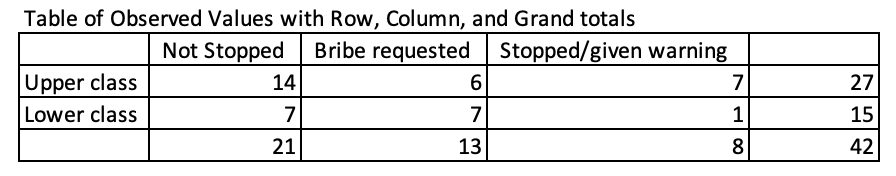
\includegraphics[scale=.90]{FoTableTotals.png}\\
	\end{center}
	
	Then, I calculated Fe for each cell using the equation:\\
	 Fe = (row total/grand total)*(column total)\\
	 
	 The table with calculated Fe in each cell is below:
	
	\begin{center}	
	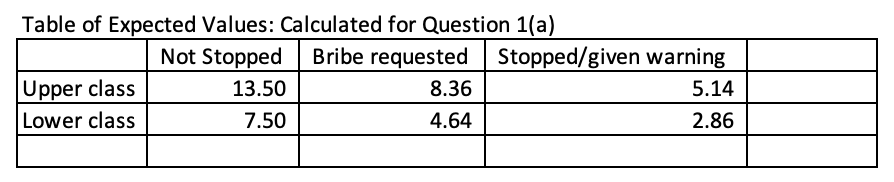
\includegraphics[scale=.90]{FeTable.png}\\
	\end{center}
	 
	Now that I have the Fe for each cell, I can calculate the $\chi^2$ test statistic.  The equation for this is:
	
	$\chi^2$ test statistic = $\sum$ ((Fo-Fe)$^2$/Fe)
	
	I manually calculated this equation (on paper), by summing the result of ((Fo-Fe)$^2$/Fe) for each cell of the table, and got the result:
	
	$\chi^2$ test statistic = 3.8269\\
	
	Note: I calculated the test statistic using values for each cell that were rounded to 4 decimal places, so the resultant test statistic might be slightly off from what I would have calculated had I done so without these rounded values. The difference should not be substantial however, and I would expect the test statistic calculated without rounded values to equal 3.8 as well.
	
	\item [(b)]
	Now calculate the p-value from the test statistic you just created (in \texttt{R}).\footnote{Remember frequency should be $>$ 5 for all cells, but let's calculate the p-value here anyway.}  What do you conclude if $\alpha = 0.1$?\\
	
	To calculate the p-value from my test statistic, I need to know my degrees of freedom.  
	
	I calculate my degrees of freedom as follows:\\
	df = (number of rows - 1)(number of columns - 1) \\
	df = (2-1)(3-1) \\
	df = (1)(2) \\
	df = 2.
	
	Next, I plug the degrees of freedom (2) and the $\chi^2$ test statistic (3.8269) into the pchisq() function in R:
	
	\lstinputlisting[language=R, firstline=58, lastline=58]{PS2_my_answers_LR.R} 
	
	Which returns a p-value from the test statistic of: 0.1475704.
	
	Because the p-value is greater than $\alpha = 0.1$ (p-value $>$ 0.1), we fail to reject the null Hypothesis (that the observations for upper and lower classes are statistically independent).
	
	\newpage
	\item [(c)] Calculate the standardized residuals for each cell and put them in the table below.
	\vspace{1cm}
	
	I now calculate the standardized residual for each cell in the table. The equation I use to calculate each cell's standardized residual is: z = (Fo - Fe)/se.\\
	se is the standard error of Fo-Fe, presuming that H0 is true, and the equation I use to calculate the standard residual for each cell is: \\
	z = ((Fo-Fe) / $\sqrt{Fe(1-row proportion)(1-column proportion)}$), or in even more detail:\\
	 z = ((Fo-Fe) / $\sqrt{Fe(1-(RowTotal/Total))
		(1-(ColumnTotal/Total))}$).  \\
	
	I calculate this for each cell and get the following standardized residuals:
	
	\begin{table}[h]
		\centering
		\begin{tabular}{l | c c c }
			& Not Stopped & Bribe requested & Stopped/given warning \\
			\\[-1.8ex] 
			\hline \\[-1.8ex]
			Upper class  & 0.3220 & -1.6437 & 1.5039 \\
			\\
			Lower class & -0.3220 & 1.6619  &  -1.5246 \\
			
		\end{tabular}
	\end{table}
	
	
	\vspace{2cm}
	\item [(d)] How might the standardized residuals help you interpret the results?  
	
	The standardized residual allows us to better see if the difference between the observed frequency and expected frequency is due to more than chance. The standardized residual of a cell is the number of standard errors (se) that Fo-Fe falls from the value we expect when H0 is true. 
	 
	 The higher (in absolute terms) a standardized residual is, is an indication of greater chance of association between the two variables (or in other words, stronger chance that the variables are not independent statistically).  Generally, if this absolute value of standardized residual in a cell is over 3, we can assume the two variables are statistically associated.  Becuase all absolute values of standardized residuals that we found in this case are less than 2, we cannot reject the null hypothesis that the variables are statistically independent for any cell.
	 
	 However, because the absolute values of the standardized residuals for Bribe requested and class, and Stopped/warned and class are closer to 2 than for not stopped and class, there is a stronger chance of association between class and whether a bribe was requested, and between class and whether the individual is warned/stopped, than there is between class and not stopped. In other words, we can say with greater confidence that class and not being stopped are statistically independent, and say with less confidence that class and bribed or class and stopped/given warning are statistically independent (though for all variables, we fail to reject claim that they are statistically independent of one another).  
	
\end{enumerate}
\newpage

\section*{Question 2 (40 points): Economics}
Chattopadhyay and Duflo were interested in whether women promote different policies than men.\footnote{Chattopadhyay and Duflo. (2004). ``Women as Policy Makers: Evidence from a Randomized Policy Experiment in India. \textit{Econometrica}. 72 (5), 1409-1443.} Answering this question with observational data is pretty difficult due to potential confounding problems (e.g. the districts that choose female politicians are likely to systematically differ in other aspects too). Hence, they exploit a randomized policy experiment in India, where since the mid-1990s, $\frac{1}{3}$ of village council heads have been randomly reserved for women. A subset of the data from West Bengal can be found at the following link: \url{https://raw.githubusercontent.com/kosukeimai/qss/master/PREDICTION/women.csv}\\

\noindent Each observation in the data set represents a village and there are two villages associated with one GP (i.e. a level of government is called "GP"). Figure~\ref{fig:women_desc} below shows the names and descriptions of the variables in the dataset. The authors hypothesize that female politicians are more likely to support policies female voters want. Researchers found that more women complain about the quality of drinking water than men. You need to estimate the effect of the reservation policy on the number of new or repaired drinking water facilities in the villages.
\vspace{.5cm}
\begin{figure}[h!]
	\caption{\footnotesize{Names and description of variables from Chattopadhyay and Duflo (2004).}}
	\vspace{.5cm}
	\centering
	\label{fig:women_desc}
	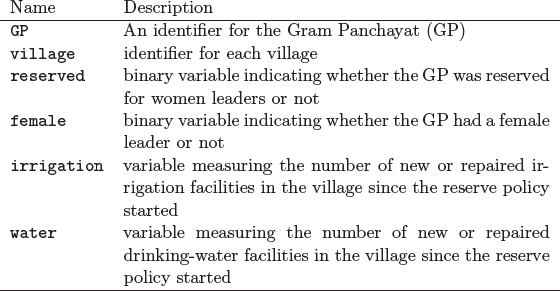
\includegraphics[width=1.1\textwidth]{women_desc.png}\\
	
\end{figure}		

\newpage

First, I loaded the csv data into R , saving it as the object "women", with the code:

	\lstinputlisting[language=R, firstline=109, lastline=109]{PS2_my_answers_LR.R} 
	

\begin{enumerate}
	\item [(a)] State a null and alternative (two-tailed) hypothesis. 
	
	Null Hypothesis (H0) = There is no association between whether a village had the reservation policy (the reserved variable) and the number of new or repaired drinking water facilities (water variable) in the village.
	
	Alternative Hypothesis (Ha) = The number of new or repaired drinking water facilities in a village is correlated with whether or not they had the reservation policy (there is a relationship) between these two variables.
	
	Note: I am using the reserved variable not the female variable, because the question is asking me to estimate the effect that the reservation policy (not explicitly whether a village has a woman leader) has on the water variable.
	
	\vspace{1cm}
	\item [(b)] Run a bivariate regression to test this hypothesis in \texttt{R} (include your code!).
	
	I wanted to test the strength of the relationship between the reserved policy (my x, or Explanatory Variable)  and the water variable (my y, or Response Variable), so I ran the code below to test my hypothesis using bivariate regression:
	
	\lstinputlisting[language=R, firstline=129, lastline=130]{PS2_my_answers_LR.R} 
	
	The summary output of this bivariate regression test was:
	
	\begin{verbatim}
Residuals:   
	 Min      1Q     Median      3Q     Max 
	 -23.991 -14.738  -7.865   2.262 316.009
	
Coefficients
              Est   Std.Error t value Pr(>|t|)    
(Intercept)    14.738  2.286  6.446   4.22e-10***
women$reserved 9.252   3.948  2.344   0.0197*  

---Signif. codes:  0 ‘***’ 0.001 ‘**’ 0.01 ‘*’ 0.05 ‘.’ 0.1 ‘ ’ 1

Residual standard error: 33.45 on 320 degrees of freedom
Multiple R-squared:  0.01688,	Adjusted R-squared:  0.0138 
F-statistic: 5.493 on 1 and 320 DF,  p-value: 0.0197
	
	\end{verbatim}
	
	\vspace{6cm}
	\item [(c)] Interpret the coefficient estimate for reservation policy. 
	
	The coefficient estimate is an estimate change in mean of the response variable (in our case, water), that we are estimated to see with a one unit change in the explanatory variable (reservation). 
	
	As seen in the above section, the coefficient estimate for reservation policy is 9.252.
	
	 We therefore interpret the coefficient estimate as: "we estimate that on average, villages with the reservation policy will have 9.252 more new or repaired drinking-water facilities than villages without the reserve policy have, since the reserve policy started."
	 
	We also interpret the p-value to test our hypothesis and add to our interpretation of the coefficient estimate. The p-value is the probability of observing this coefficient estimate or one that is more extreme if the null hypothesis is actually correct. A low p value indicates that we can reject our null hypothesis.  The p-value for this regression test is 0.0197. This is a low p-value (lower at least then 0.05, which is often used as the "benchmark"). Thus, this bivariate regression output leads us to reject our null hypothesis, that there is no relationship / association between the two variables (reservation policy and water). Using these statistics, we predict villages with the policy to have introduced more (on average) new / repaired drinking water facilities than those without the policy. 
	

	
	
\end{enumerate}

\end{document}
